% !TEX root = ../report.tex
\task{2B}{Dynamic I-RRIP}

\subsection{Leader sets and decision logic}

\textbf{Mechanism.} A few L2C sets, the \emph{leaders}, always run SRRIP. In the leaders we count instruction accesses, instruction misses, all accesses and all misses, over demand traffic only (writebacks and prefetches are not counted). The other sets, the \emph{followers}, run I-RRIP (from Task 2A) or SRRIP, as decided from the leaders' counts. Every line records on fill whether it is an instruction line, in every set and in both modes, so a follower that switches mode keeps valid state; both modes use the same 2-bit RRPV scale.

\textbf{Decision.} We use the formula from the problem statement,
\[
  r = \frac{\text{instr.\ accesses} + \text{instr.\ misses}}{\text{total accesses} + \text{total misses}},
\]
and the followers run I-RRIP when $r > T$, SRRIP otherwise.

\textbf{Epochs.} The decision is made once per \emph{epoch}, every $E$ demand accesses to the leaders. After each decision the four counters are halved. This has the effect of giving greater weight to recent epochs so that counters don't converge to the whole-run average and stop the policy from ever switching. \textbf{We finally use 1024 epochs.}

\textbf{Why the leaders run SRRIP.} If the leaders ran I-RRIP, the ratio we mentioned would be skewed anyway. It would require a more complex interpretation of the threshold (perhaps simple threshold will not even suffice). Reason: I-RRIP removes instruction misses, which lowers $r$ and can switch the followers to SRRIP, which raises instruction misses again. With SRRIP leaders, $r$ measures the workload in an easy to interpret manner so we can set a direct threshold.

\textbf{Leader placement choice.} There are $N$ leaders among the 1024 sets, and rule is: \textbf{set $s$ is a leader when its low $k$ index bits equal the next $k$ bits} (it is called ``complement placement''), where $1024/2^k = N$ (for $N = 32$: \texttt{(s \& 31) == ((s >> 5) \& 31)}). Leaders then sit at different offsets in the index, so an access pattern that maps only to some set offsets cannot dominate the sample. We also compared this placement with two others (low index bits all 0, and the first $N$ sets): the speedups differ by less than 0.1\% for $T \le 0.25$ (Table~\ref{tab:t2b-place}).

\textbf{How many leaders.} Each leader set gives up on some I-RRIP gain, since it always runs SRRIP. With 8 or 16 leaders the policy makes no SRRIP decision after warmup, so their loss against static I-RRIP (0.02\% and 0.04\%, Table~\ref{tab:t2b-leaders}) is the cost of the leader sets alone. More leaders would only help in getting a less noisy estimate for $r$; but in our runs we saw this never occured. More leaders also make each epoch shorter in instructions (an epoch counts leader accesses), so the decision follows shorter dips in $r$ and switches more often, which costs speedup: 32 and 64 leaders switch to SRRIP on Trace2 and Trace3 and lose 0.44\% and 0.52\% (see the sensitivity study below). \textbf{We use 8 leaders finally}.

\textbf{Final parameters} (the code defaults): 8 leaders, complement placement, $E = 1024$ leader accesses, $T = 0.15$, hysteresis $h = 0.05$ (see the extension below).

\subsection{Sensitivity study}

We did ``pilot'' runs over wider ranges (8--256 leaders, epochs of 128--8192, $T$ from 0 to 1) to find some reasonable ranges to do intensive testing: $T$ below 0.15 changes nothing, and from $T = 0.7$ on every trace runs SRRIP throughout. The threshold, leader, epoch and placement sweeps use no hysteresis ($h = 0$); hysteresis is studied seperately later. All results are averages over the three traces; the ratio columns are each MPKI relative to static I-RRIP (geometric mean of the per-trace ratios).

\textbf{Threshold $T$} (8 leaders, $E = 512$):

\begin{table}[H]
\centering
\small
% Generated by report/task2b.py from data/. Do not edit by hand.
\begin{tabular}{@{}lrrrrrrrr@{}}
\toprule
& & & \multicolumn{3}{c}{Load MPKI} & \multicolumn{3}{c}{MPKI ratio to I-RRIP} \\
\cmidrule(lr){4-6} \cmidrule(l){7-9}
$T$ & IPC & Speedup & L2C & Instr. & Data & L2C & Instr. & Data \\
\midrule
SRRIP & 0.2886 & 1.0004 & 15.81 & 9.85 & 5.96 & 1.098 & 1.694 & 0.766 \\
I-RRIP & 0.2943 & 1.0216 & 13.91 & 5.76 & 8.14 & 1.000 & 1.000 & 1.000 \\
\midrule
0 & 0.2942 & 1.0214 & 13.91 & 5.79 & 8.12 & 1.000 & 1.005 & 0.997 \\
0.15 & 0.2942 & 1.0213 & 13.90 & 5.79 & 8.11 & 1.000 & 1.005 & 0.996 \\
0.25 & 0.2940 & 1.0208 & 13.91 & 5.81 & 8.10 & 1.001 & 1.029 & 0.992 \\
0.4 & 0.2925 & 1.0159 & 14.15 & 6.21 & 7.94 & 1.021 & 1.161 & 0.972 \\
0.5 & 0.2916 & 1.0123 & 14.09 & 6.78 & 7.31 & 1.020 & 1.258 & 0.905 \\
\bottomrule
\end{tabular}

\caption{Threshold sweep. Speedup over LRU (geometric mean); MPKI is the arithmetic mean.}\label{tab:t2b-thresh}
\end{table}

\begin{figure}[H]
\centering
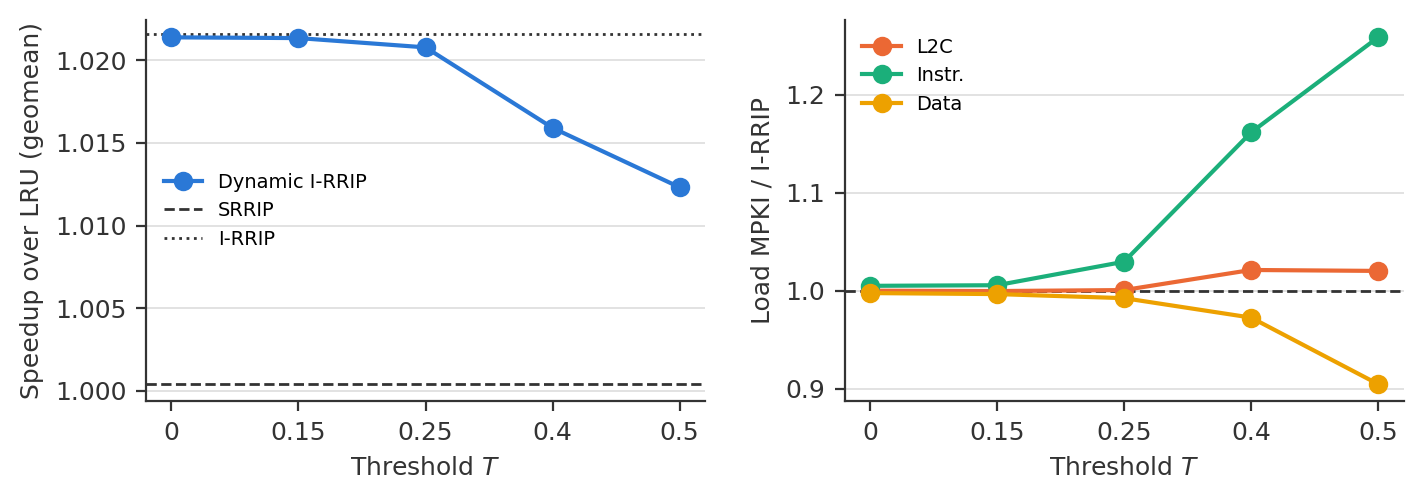
\includegraphics[width=0.85\textwidth]{t2b_thresh.png}
\caption{Threshold sweep: speedup over LRU, and each MPKI relative to I-RRIP.}
\end{figure}

\textbf{Speedup falls as $T$ rises}: from 1.0214 at $T = 0$ to 1.0123 at $T = 0.5$. A higher $T$ means more epochs decide to run SRRIP; e.g. at $T = 0.5$, Trace1 runs SRRIP in 10 of its 14 decisions. SRRIP epochs raise instruction MPKI more than they lower data MPKI, and as Task 2A showed, instruction misses cost more. The same holds at every leader count and epoch length we ran.

\textbf{Leader count} ($T = 0.15$, $E = 1024$): Table~\ref{tab:t2b-leaders}, discussed above.

\begin{table}[H]
\centering
\small
% Generated by report/task2b.py from data/. Do not edit by hand.
\begin{tabular}{@{}lrrrrrrrr@{}}
\toprule
& & & \multicolumn{3}{c}{Load MPKI} & \multicolumn{3}{c}{MPKI ratio to I-RRIP} \\
\cmidrule(lr){4-6} \cmidrule(l){7-9}
Leaders & IPC & Speedup & L2C & Instr. & Data & L2C & Instr. & Data \\
\midrule
SRRIP & 0.2886 & 1.0004 & 15.81 & 9.85 & 5.96 & 1.098 & 1.694 & 0.766 \\
I-RRIP & 0.2943 & 1.0216 & 13.91 & 5.76 & 8.14 & 1.000 & 1.000 & 1.000 \\
\midrule
8 & 0.2942 & 1.0214 & 13.91 & 5.79 & 8.12 & 1.000 & 1.005 & 0.997 \\
16 & 0.2942 & 1.0212 & 13.94 & 5.83 & 8.10 & 1.002 & 1.013 & 0.996 \\
32 & 0.2941 & 1.0209 & 13.96 & 5.87 & 8.08 & 1.003 & 1.021 & 0.993 \\
64 & 0.2938 & 1.0199 & 14.02 & 6.01 & 8.01 & 1.007 & 1.047 & 0.986 \\
\bottomrule
\end{tabular}

\caption{Leader count sweep ($T = 0.15$, $E = 1024$). 8 and 16 leaders make no SRRIP decision after warmup, so their loss against I-RRIP is the cost of the leader sets; 32 and 64 leaders switch to SRRIP on Trace2 and Trace3.}\label{tab:t2b-leaders}
\end{table}

\begin{figure}[H]
\centering
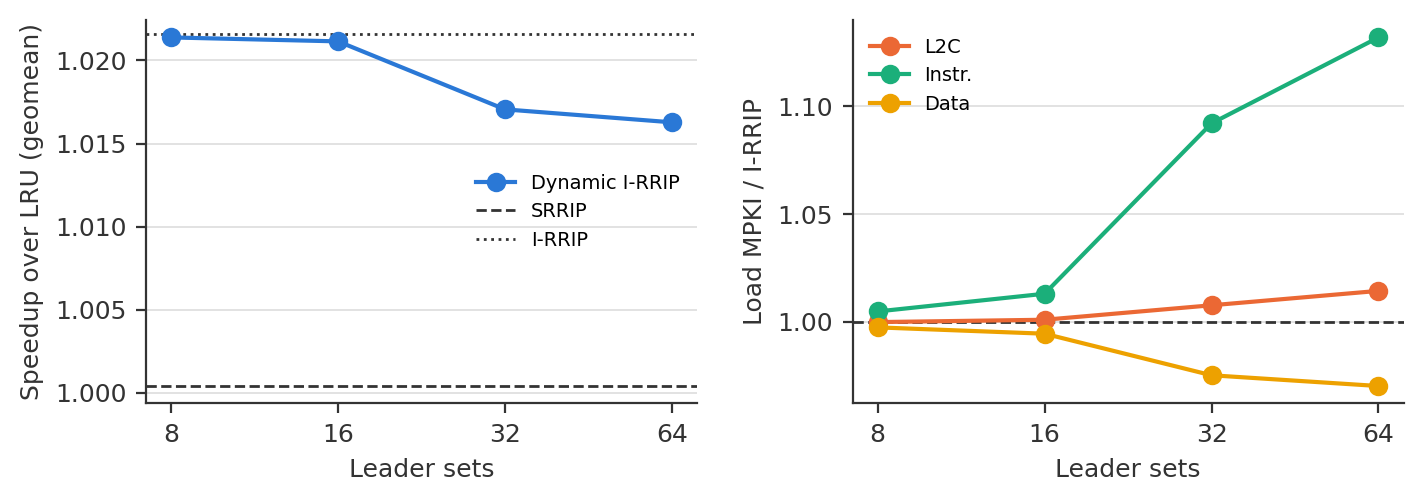
\includegraphics[width=0.85\textwidth]{t2b_leaders.png}
\caption{Leader count sweep: speedup over LRU, and each MPKI relative to I-RRIP.}
\end{figure}

\textbf{Epoch length} (32 leaders, $T = 0.15$):

\begin{table}[H]
\centering
\small
% Generated by report/task2b.py from data/. Do not edit by hand.
\begin{tabular}{@{}lrrrrrrrr@{}}
\toprule
& & & \multicolumn{3}{c}{Load MPKI} & \multicolumn{3}{c}{MPKI ratio to I-RRIP} \\
\cmidrule(lr){4-6} \cmidrule(l){7-9}
Epoch & IPC & Speedup & L2C & Instr. & Data & L2C & Instr. & Data \\
\midrule
SRRIP & 0.2886 & 1.0004 & 15.81 & 9.85 & 5.96 & 1.098 & 1.694 & 0.766 \\
I-RRIP & 0.2943 & 1.0216 & 13.91 & 5.76 & 8.14 & 1.000 & 1.000 & 1.000 \\
\midrule
512 & 0.2927 & 1.0166 & 13.99 & 6.04 & 7.94 & 1.010 & 1.112 & 0.975 \\
1024 & 0.2929 & 1.0171 & 14.02 & 6.07 & 7.94 & 1.008 & 1.092 & 0.975 \\
2048 & 0.2941 & 1.0208 & 13.94 & 5.88 & 8.07 & 1.002 & 1.022 & 0.992 \\
\bottomrule
\end{tabular}

\caption{Epoch length sweep, in leader accesses.}
\end{table}

\begin{figure}[H]
\centering
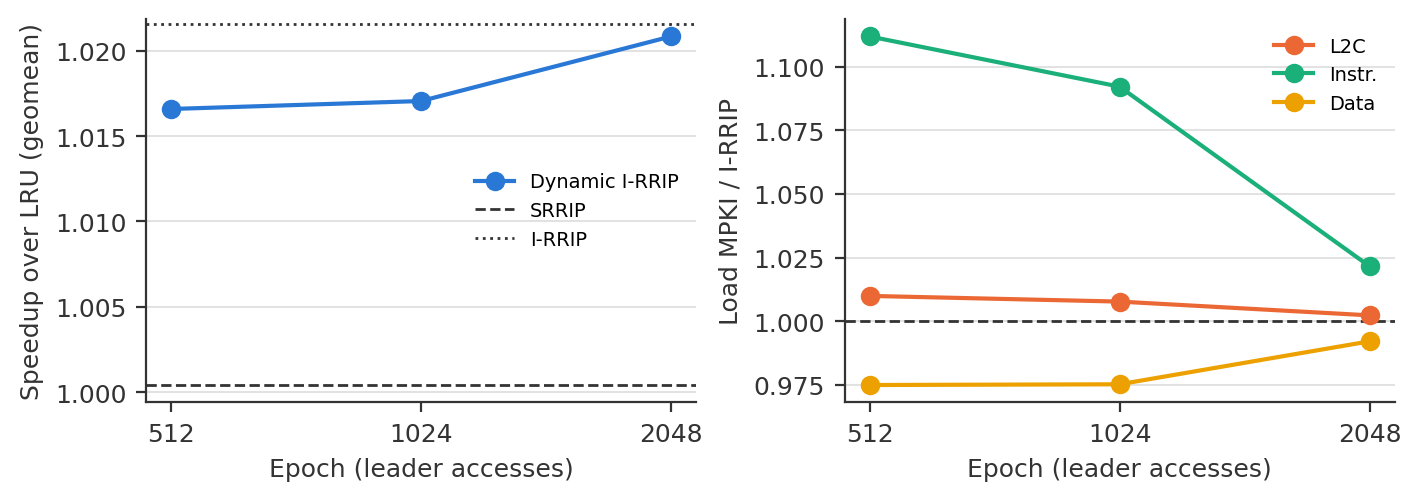
\includegraphics[width=0.85\textwidth]{t2b_epoch.png}
\caption{Epoch length sweep: speedup over LRU, and each MPKI relative to I-RRIP.}
\end{figure}

Longer epochs are better (1.0166, 1.0171, 1.0208), but only because they decide less often: each decision averages $r$ over more instructions, so short dips no longer reach SRRIP. At $E = 2048$ no trace makes an SRRIP decision after warmup.

\textbf{Placement} (32 leaders, $E = 1024$):

\begin{table}[H]
\centering
\small
% Generated by report/task2b.py from data/. Do not edit by hand.
\begin{tabular}{@{}lrrr@{}}
\toprule
$T$ & complement select & low bits = 0 & first sets \\
\midrule
0 & 1.0209 & 1.0206 & 1.0207 \\
0.15 & 1.0171 & 1.0173 & 1.0165 \\
0.25 & 1.0163 & 1.0161 & 1.0160 \\
0.4 & 1.0144 & 1.0126 & 1.0133 \\
0.5 & 1.0124 & 1.0108 & 1.0121 \\
\bottomrule
\end{tabular}

\caption{Speedup over LRU for the three leader placements.}\label{tab:t2b-place}
\end{table}

\textbf{Why switching does not pay.} The ratio does vary within a trace: with 32 leaders and $E = 1024$, $r$ on Trace2 ranges from 0.07 to 0.70 across epochs. But no configuration we ran beats static I-RRIP on average, and the more decisions choose SRRIP, the lower the speedup. The ratio measures how much of the L2 traffic is instructions, not which policy is better: the epochs where $r$ is low are not epochs where SRRIP wins, since switching to SRRIP in them lowered speedup. A short visit to SRRIP also costs more than its share of the run: on Trace3, 2 SRRIP decisions out of 7 lose 0.61\% (16 leaders, $E = 512$), against 0.84\% for SRRIP over the whole run. The damage outlasts the switch back to I-RRIP. \brt{why it lasts is not measured; candidates: instruction lines evicted during the SRRIP epoch, or data lines left at RRPV 0 by SRRIP's promotion.}

\textbf{Extension: hysteresis.} The problem statement allows extending the formula. With a single threshold, a small dip of $r$ just below $T$ flips the mode, and those switches cost speedup. We added a band of $\pm h$: switch to I-RRIP only when $r > T + h$, and to SRRIP only when $r \le T - h$.

\begin{table}[H]
\centering
\small
% Generated by report/task2b.py from data/. Do not edit by hand.
\begin{tabular}{@{}lrrrrrrrr@{}}
\toprule
& & & \multicolumn{3}{c}{Load MPKI} & \multicolumn{3}{c}{MPKI ratio to I-RRIP} \\
\cmidrule(lr){4-6} \cmidrule(l){7-9}
$h$ & IPC & Speedup & L2C & Instr. & Data & L2C & Instr. & Data \\
\midrule
SRRIP & 0.2886 & 1.0004 & 15.81 & 9.85 & 5.96 & 1.098 & 1.694 & 0.766 \\
I-RRIP & 0.2943 & 1.0216 & 13.91 & 5.76 & 8.14 & 1.000 & 1.000 & 1.000 \\
\midrule
0 & 0.2929 & 1.0171 & 14.02 & 6.07 & 7.94 & 1.008 & 1.092 & 0.975 \\
0.05 & 0.2939 & 1.0200 & 13.91 & 5.93 & 7.98 & 1.000 & 1.028 & 0.984 \\
0.1 & 0.2941 & 1.0208 & 13.94 & 5.88 & 8.07 & 1.002 & 1.022 & 0.992 \\
\bottomrule
\end{tabular}

\caption{Hysteresis sweep (32 leaders, $E = 1024$, $T = 0.15$).}
\end{table}

\begin{figure}[H]
\centering
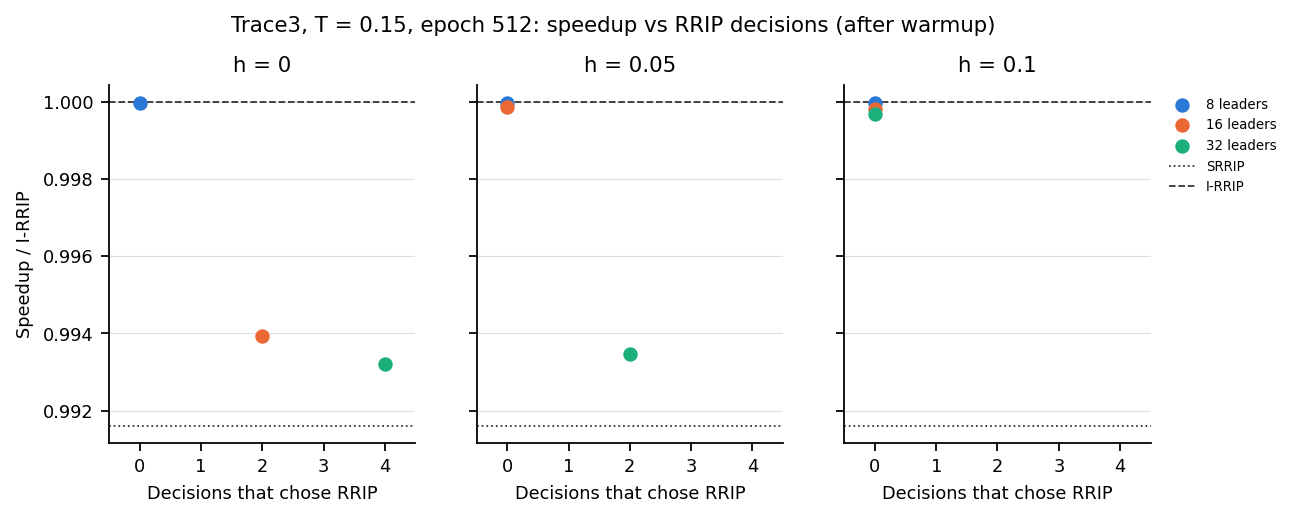
\includegraphics[width=0.9\textwidth]{t2b_hyst_decisions.png}
\caption{Trace3, $T = 0.15$, $E = 512$: speedup relative to I-RRIP against the number of decisions after warmup that chose SRRIP, one panel per $h$, one point per leader count.}
\end{figure}

Hysteresis raises speedup (1.0171, 1.0200, 1.0208 for $h = 0$, 0.05, 0.1), but only by removing SRRIP decisions: in the figure, speedup returns to I-RRIP's only for the points with no SRRIP decision left, and no point with SRRIP decisions sits above one without. Since every SRRIP decision the ratio makes costs speedup on these traces, hysteresis can at best make the policy never switch. It did not improve on static I-RRIP. We still keep $h = 0.05$ in the final configuration. There it gives results identical to $h = 0$, since the policy makes no SRRIP decision either way. Among the configurations that switch, it raised speedup by 0.2--0.3\% in two (16 leaders at $E = 512$, 32 leaders at $E = 1024$) and changed it by at most 0.03\% in the other three. It guards against noisy switching on workloads whose $r$ stays near $T$.

\subsection{Results}

\begin{table}[H]
\centering
\small
% Generated by report/task2b.py from data/. Do not edit by hand.
\begin{tabular}{@{}llrrrrr@{}}
\toprule
Trace & Policy & IPC & Speedup & L2C & L2C instr. & L2C data \\
\midrule
Trace1 & LRU (baseline) & 0.2323 & 1.0000 & 17.70 & 10.34 & 7.36 \\
 & SRRIP & 0.2322 & 0.9995 & 17.64 & 10.56 & 7.08 \\
 & I-RRIP & 0.2339 & 1.0068 & 18.60 & 8.98 & 9.62 \\
 & Dynamic I-RRIP & 0.2339 & 1.0067 & 18.59 & 8.99 & 9.60 \\
\midrule
Trace2 & LRU (baseline) & 0.2512 & 1.0000 & 27.36 & 18.85 & 8.50 \\
 & SRRIP & 0.2518 & 1.0026 & 25.75 & 17.78 & 7.96 \\
 & I-RRIP & 0.2639 & 1.0509 & 19.25 & 7.63 & 11.62 \\
 & Dynamic I-RRIP & 0.2638 & 1.0504 & 19.27 & 7.69 & 11.58 \\
\midrule
Trace3 & LRU (baseline) & 0.3821 & 1.0000 & 3.95 & 1.12 & 2.83 \\
 & SRRIP & 0.3817 & 0.9991 & 4.04 & 1.20 & 2.84 \\
 & I-RRIP & 0.3850 & 1.0076 & 3.87 & 0.67 & 3.19 \\
 & Dynamic I-RRIP & 0.3850 & 1.0076 & 3.86 & 0.68 & 3.19 \\
\midrule
Mean & LRU (baseline) & 0.2885 & 1.0000 & 16.34 & 10.11 & 6.23 \\
 & SRRIP & 0.2886 & 1.0004 & 15.81 & 9.85 & 5.96 \\
 & I-RRIP & 0.2943 & 1.0216 & 13.91 & 5.76 & 8.14 \\
 & Dynamic I-RRIP & 0.2942 & 1.0214 & 13.91 & 5.79 & 8.12 \\
\bottomrule
\end{tabular}

\caption{IPC, speedup over LRU, and L2C load MPKI (total, instruction, data) of Dynamic I-RRIP with the final parameters. Mean: geometric for speedup, arithmetic otherwise.}
\end{table}

\begin{figure}[H]
\centering
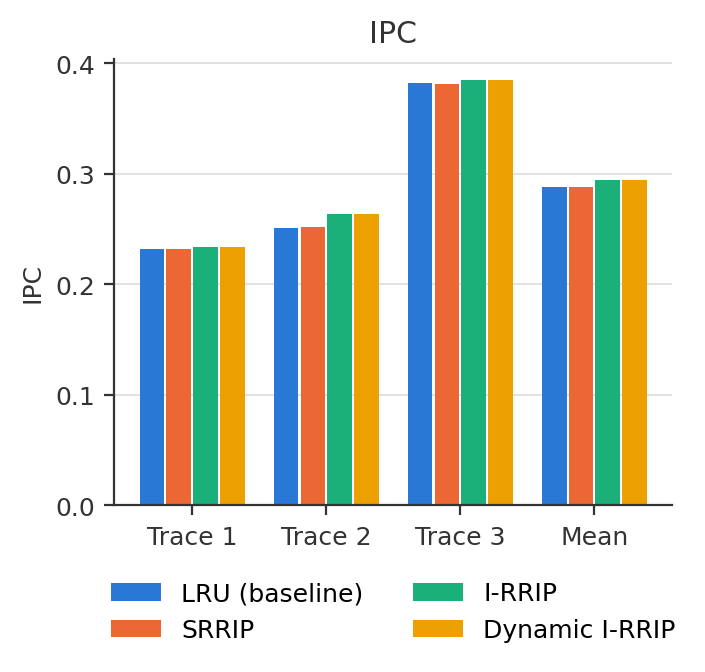
\includegraphics[width=0.32\textwidth]{t2b_ipc.png}\hfill
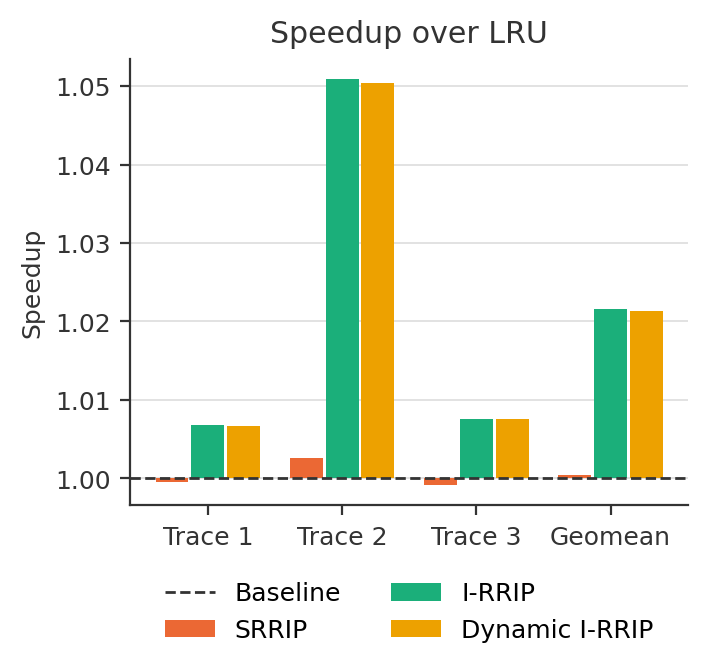
\includegraphics[width=0.32\textwidth]{t2b_speedup.png}\hfill
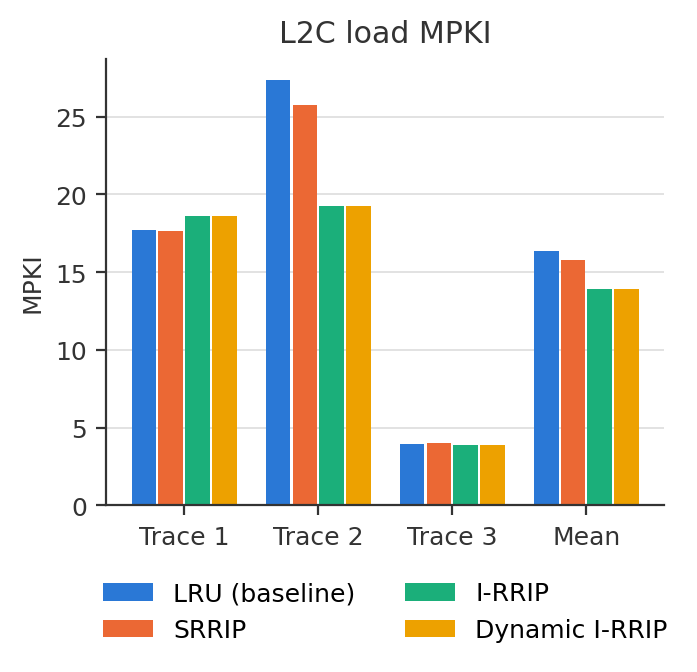
\includegraphics[width=0.32\textwidth]{t2b_mpki.png}\\[0.4em]
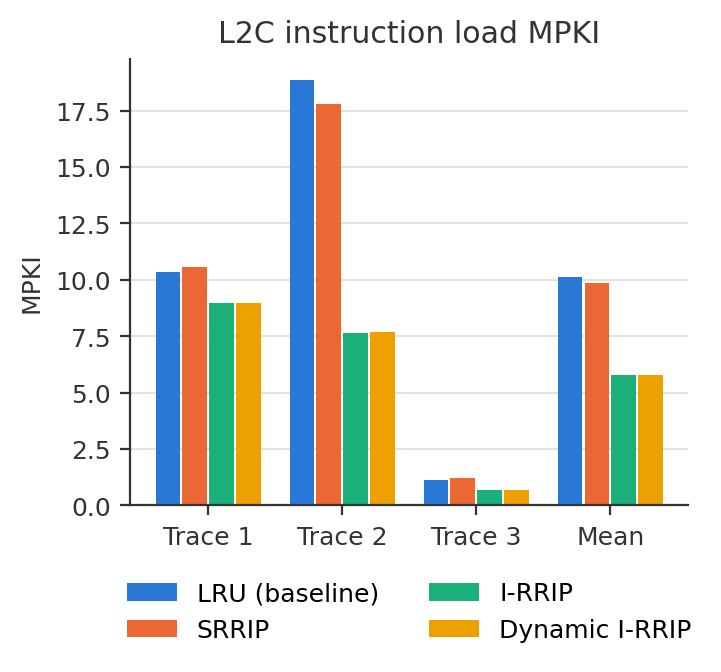
\includegraphics[width=0.32\textwidth]{t2b_mpki_instr.png}\hspace{0.02\textwidth}
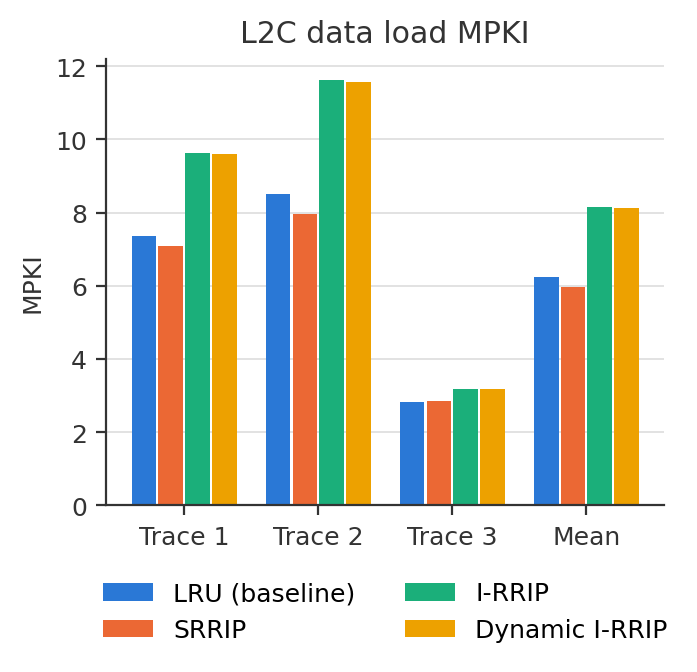
\includegraphics[width=0.32\textwidth]{t2b_mpki_data.png}
\caption{IPC, speedup over LRU (dashed line), and L2C load MPKI per trace.}
\end{figure}

Dynamic I-RRIP reaches a speedup of 1.0214 over LRU, against 1.0216 for static I-RRIP, and the same L2C load MPKI (13.91). With the final parameters it makes no SRRIP decision after warmup on any trace: at every decision $r$ is at least 0.46 on Trace1, 0.28 on Trace2 and 0.39 on Trace3, well above $T = 0.15$. So on these traces it behaves as static I-RRIP minus the cost of the 8 leader sets (0.02\%). It decides slowly: with 8 leaders, an epoch of 1024 leader accesses gives 7, 13 and 2 decisions over the 25M simulated instructions of Trace1, Trace2 and Trace3. It switches to SRRIP only when $r$, as kept by the halving counters, is $T - h = 0.10$ or less at a decision, and back to I-RRIP only when $r$ exceeds $T + h = 0.20$.
